\section{Background and System Description}\label{sec:aggregation:background}
In this section we describe different bandwidth aggregation approaches in praxis and present related work on the performance evaluation of bandwidth aggregation systems.
In addition, we describe our system model of bandwidth aggregation systems with offloading policy.

\subsection{Bandwidth Aggregation Approaches}\label{sec:aggregation:background:aggr}

The principle of sharing or offloading between multiple Internet access links is already widely used by commercial services as well as research work. WiFi-sharing communities like Fon\footnote{\url{http://www.fon.com}}, Karma\footnote{\url{https://yourkarma.com/}}, WeFi\footnote{\url{http://wefi.com/}}, and Boingo\footnote{\url{http://www.boingo.com/}} offer access to an alternative Internet link (WiFi instead of mobile), which provides a faster access bandwidth and reduces the load on stressed mobile networks. With respect to this so called ``WiFi offloading'', the research community investigated incentives and algorithms for access sharing \cite{mamatas2010incentives}, and ubiquitous WiFi access architectures for deployment in metropolitan areas \cite{sastry2007architecting, vidales2009metropolitan}. Moreover, \cite{lafuente2011flexible,donelson2012patent,seufert2013horst} describe systems for trust-based WiFi password sharing via an online social network (OSN) app. WiFi sharing is not a legal vacuum and a first exemplary overview on Swiss and French rights and obligations was given in \cite{camponovo2005wlan} but must be treated with caution due to international differences and interim law revisions.
The opposite concept to Wifi offloading, i.e., WiFi onloading, is presented in \cite{rossi20133gol}. The idea is to utilize different peaks in mobile and fixed networks to onload data to the mobile network to support applications on short time scales (e.g., prebuffering of videos, asymmetric data uploads).

%Bewifi
An access link sharing concept, which goes beyond pure offloading, is BeWifi, which was developed by Telefonica \cite{goma2013patent} and builds on previous works about backhaul capacity aggregation \cite{kandula2008fatvap,giustiniano2010fair}. BeWifi uses modified access points, which act as normal access points until their clients saturate more than 80\% of the backhaul capacity. Then, the access point will scan for close access points, which will provide additional bandwidth if their utilization is below 70\%. Backhaul capacity and utilization are announced by each access point via beacon frames. Instead of introducing a secondary WiFi radio, BeWifi uses time-division multiple access (TDMA) and the 802.11 network allocation vector (NAV) to connect to neighboring access points for bandwidth aggregation in a round robin fashion with a weighted proportional fairness schedule.

% The client-based solution requires driver modifications on the wireless clients.
% Each wireless client needs to feature a virtualized wireless card.
% This implies that for a commercial deployment the operating system and wireless driver of every WiFi client needs to be modified, which would produce a high amount of costs.
% %As one may realize, the cost of such an approach is absolutely prohibitive.
% The problem of the diversity of devices that need to be modified can be solved
% by deploying the aggregation scheme in the access points, which are usually provided by ISPs.
% However, current methods to perform aggregation with single-radio devices are not meant to be used in APs.
% Introducing a secondary WiFi radio in the APs could provide a technical solution, but it increases the cost of a device that is subsidized by the ISP, making the solution impracticable.

\reffig{fig:aggregation:background:aggr} shows a client-based and an access point solution for the bandwidth aggregation proposed in \cite{goma2013patent}.
The state of the art client-based system proposes to use a TDMA based access strategy for accessing selected access points in range in a round robin fashion, i.e., no concurrent data transmission via different frequencies is taking place.
The system utilizes inband signaling, a switching frequency of 100ms and requires less than 1.5ms for switching.
%The state of the art client-based aggregation schemes propose the use of TDMA to enable a single-radio client to connect to all the neighboring access points, as in \reffig{fig:aggregation:background:aggrclient} regardless of their frequency of operation. Over cycles of 100 ms the wireless client sequentially connects to all selected access points within range in a round robin fashion.
%The system utilizes inband signaling and requires less than 1.5 ms for switching.
Using the standard 802.11 power saving feature, a client is able to notify its absence to the access points it is connected to, so that they buffer packets directed to it.
A client performing aggregation appears to be sleeping in all access points but the one that is currently scheduled in the round robin cycle.
%No concurrent data transmission via different frequencies is taking place.
The access-point-based solution can be mapped to the client-based solution, if an access point acts as access point to its clients, and as a client to neighboring access points.
%single-radio AP that acts as an AP to its clients, and as a client to neighboring APs, and show that the problem can be mapped to the client-based solutions allowing the same optimization objectives

%acts as an AP and as a client of a neighboring AP
%the APs transmit on different channels
%The client-based solution is able to fully aggregate the available capacity of the
%backhaul links for a wider range of wireless channel capacities.
%their need for client modifications makes their deployment cost prohibitive.
%To unleash the potential of those solutions, the present invention provides and implements a system that can approach the benefits of client-based solutions requiring modifications only on the APs

\begin{figure*}[tb]
    \centering
    \begin{subfigure}[t]{0.5\textwidth}
        \centering
        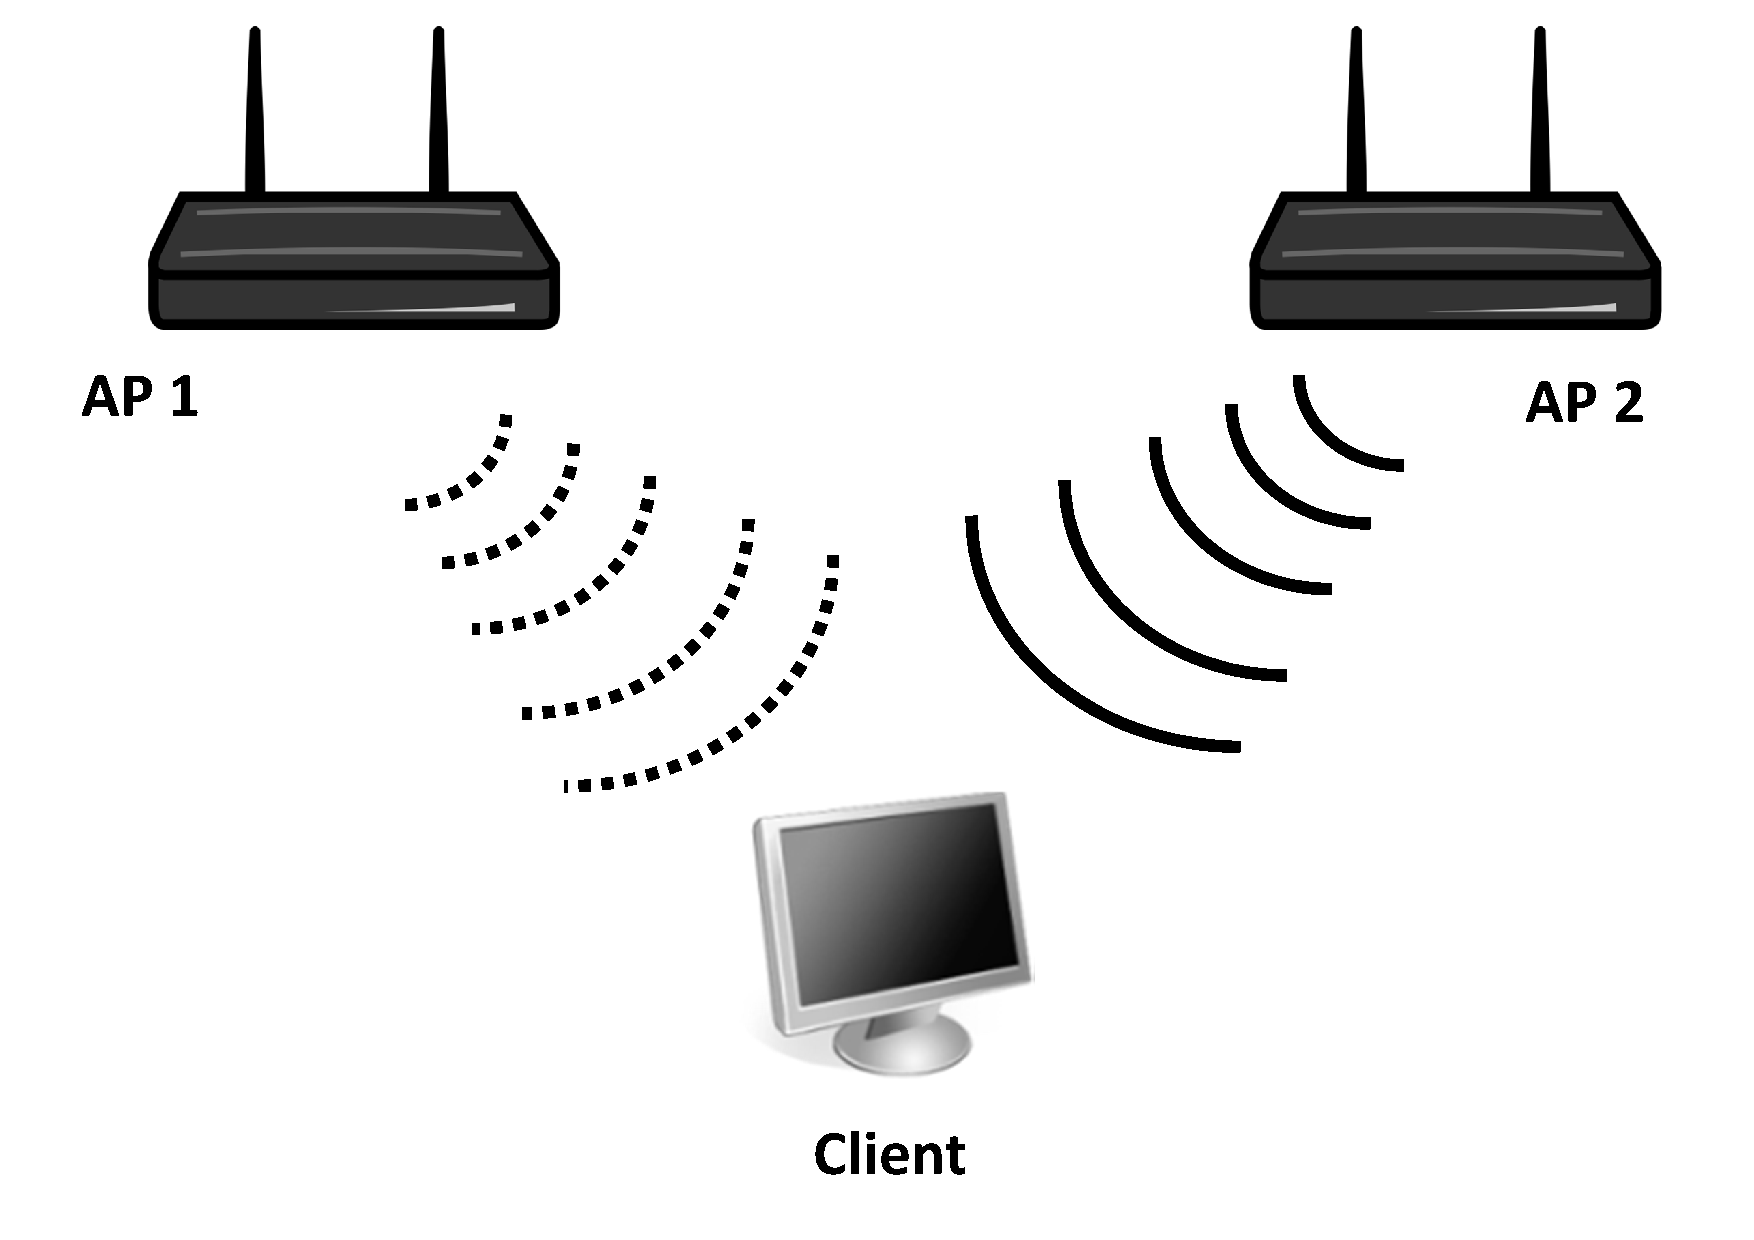
\includegraphics[width=.9\textwidth]{aggregation/background/figures/aggr_client_sw}
        \caption{Client-based}
				\label{fig:aggregation:background:aggrclient}
    \end{subfigure}%
    ~
    \begin{subfigure}[t]{0.5\textwidth}
        \centering
        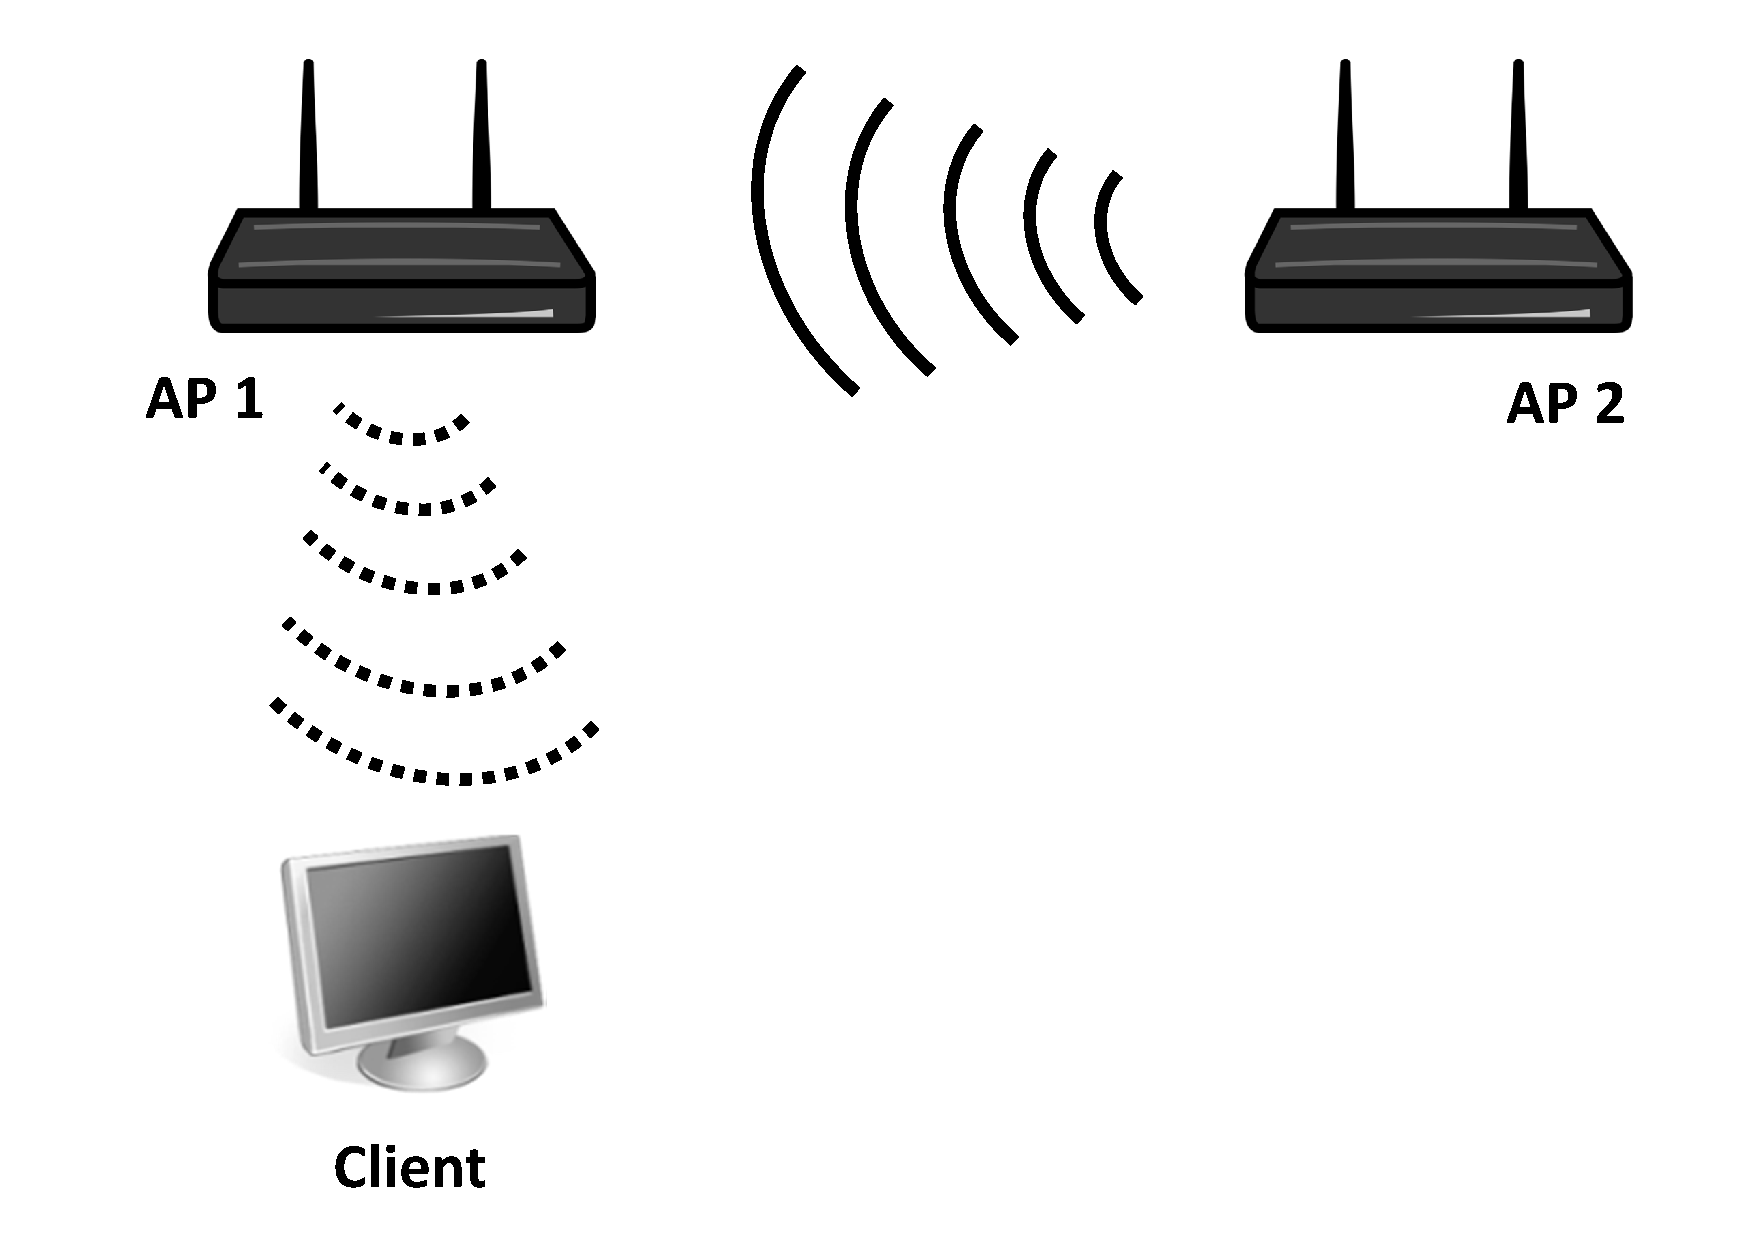
\includegraphics[width=.9\textwidth]{aggregation/background/figures/aggr_ap_sw}
        \caption{Access-point-based}
				\label{fig:aggregation:background:aggrap}
    \end{subfigure}
    \caption{Client-based and access-point-based solution for bandwidth aggregation.}
		\label{fig:aggregation:background:aggr}
\end{figure*}

From a technical perspective, bandwidth sharing and offloading are enabled by implementing handovers and/or multipath connections, which are well covered in research. \cite{gonzalez2013radio,paasch2012exploring,chen2013energy} show the feasibility of multipath TCP for handovers between mobile and WiFi networks in the current Internet and \cite{khadraoui2014survey} describes available features for mobile traffic offloading. Futhermore, \cite{gladisch2014survey} gives an overview on approaches that enable mobility and multihoming.
%In \cite{shifrin2010c3} a collaborative token bucket algorithm, which implements an effective distribution of the transmission rates is analyzed to evaluate the performance of wireless ad-hoc and mesh networks.

\subsection{Perfomance Models for Bandwidth Aggregation Systems}\label{sec:aggregation:background:models}

Theoretically, bandwidth sharing between WiFi access points can be considered as load sharing among systems.
Generally load sharing systems can be classified in partitioning, partial sharing and complete sharing systems.
Partitioning systems work completely independent from each other.
Each system has its own queue and buffer space and processes only requests arriving at its queue.
Complete sharing systems have a shared queue and buffer space. When processed, a request in the shared queue is assigned to the system which is currently least loaded.

Partial sharing systems have their own queues, but may offload requests to other systems if they are overloaded, or process requests from other overloaded systems.
Different partial sharing or complete sharing models have been investigated in literature.
In \cite{trangia1993trunk} the bandwidth usage by different services in a broadband system in complete sharing and partial sharing mode with trunk reservation is investigated.
Multidimensional Markov chains are used in \cite{chen2002performance,zhang2006dynamic,ke2010performance} to evaluate the performance of cellular network systems with different service categories.
The blocking probability of a complete sharing system has been approximated in \cite{kaufman1992blocking}.
This approximation is used in \cite{fodor2007bounding} to evaluate the performance of mobile networks with code division multiplexing supporting elastic services.
However, none of the models can be used to seamlessly evaluate the performance of systems between partitioning and complete sharing.

Thus, we develop a model based on a two dimensional Markov chain with thresholds to study the transition of blocking probabilities of partitioned, partial sharing, and complete sharing systems.
%The Markov model is limited to two access links only.
This limits its applicability, since the number of average WiFi access points visible to clients is much higher in densely-populated areas.
In densely-populated areas bandwidth of a high number of WiFi access points is aggregated. In this case an assessment with the Markov model  is not possible, since it is limited to two access links. An extension of the Markov model to $m$ dimensions would require solving an equation system with $n^m$ equations, which is computationally too complex.
Therefore, we extend the model to be applicable to multiple access links by utilizing a fixed point approximation.

The fixed point approximation is used to reduce the m-dimensional Markov chain to one dimension similar to \cite{trangia1992polling, staehle2002approximation}, where the approach is used for analytic models for polling systems and the interference distribution in UMTS networks, respectively.
The underlying Markov chain highly differs from existing fix-point approaches, since it considers support and offloading thresholds.
To the best of our knowledge this is also the first work that considers an inner and an outer composite system to apply the fixed point analysis in heterogeneous load conditions.

%multipath transmissions
%Multipath transmissions?
%von hossi:
% Survey on Mobility and Multihoming in Future Internet: http://link.springer.com/article/10.1007/s11277-012-0898-6#page-1
% A Survey of Available Features for Mobile Traffic Offload: http://ieeexplore.ieee.org/stamp/stamp.jsp?tp=&arnumber=6843152
% Exploring Mobile/WiFi Handover with Multipath TCP: http://inl.info.ucl.ac.be/system/files/cell06-paasch.pdf
% An Energy-aware Multipath-TCP-based Content Delivery Scheme in Heterogeneous Wireless Networks: http://www.eeng.dcu.ie/~munteang/papers/2013_WCNC_SC.pdf
% Radio access considerations for data offloading with multipath TCP in cellular/WiFi networks: http://ieeexplore.ieee.org/xpl/freeabs_all.jsp?arnumber=6496709&abstractAccess=no&userType=inst

\subsection{System Model}


For simplicity and mathematical tractability we make assumptions on the link capacities and the service rates of bandwidth fractions. This allows analytic performance evaluation of bandwidth aggregation systems with offloading policy and understanding its characteristics.


%\newtheorem{amp4}[amp1]{Assumption}\label{amp:traffic}
%\begin{amp4}
%	The arrivals of traffic bursts follow a Poisson process.
%\end{amp4}

%There are different effects in real systems, which are not considered in the model.

\newtheorem{amp1}{Assumption}\label{amp:switching}
\begin{amp1}
	The switching time to another access link is zero.
\end{amp1}
In practice, TDMA is used to aggregate the bandwidth of two access points operating on different channels.
During the time in which the client is switching frequencies, it cannot send or transmit data. This time is called switching time and for state of the art systems it is 1.5ms \cite{goma2013patent}.
This switching time slightly decreases the effective throughput of the system.
Signaling among the cooperating access points is necessary to report the current load and the offloading state.
The messages exchanged produce a signaling overhead, which can limit the performance of the system.
In practice APs announce their backhaul link capacity through Beacon frames, as well as their available-for-aggregation throughput, i.e. the part of their capacity that is not utilized by their clients \cite{goma2013patent}.
However, in \cite{goma2013patent} the aggregate throughput remains almost constant across the different experiments, indicating that the overhead of switching and signaling is fixed and only slightly impacts the overall throughput.
\newtheorem{amp2}[amp1]{Assumption}\label{amp:aggrlimit}
\begin{amp2}
	The wireless channels are clean.
\end{amp2}
Interference can limit the capacity of the wireless links.
The effect of the channel quality on the aggregation capacity is evaluated in \cite{goma2013patent}.
To account for a bad channel quality in our model, the link capacity can be reduced accordingly.

\newtheorem{amp3}[amp1]{Assumption}\label{amp:servicetimes}
\begin{amp3}
	The service time of bandwidth fractions follows a negative exponential distribution.
\end{amp3}
%In practice, the link throughput has low variations which makes the service time of traffic bursts more deterministic.
%As shown in \cite{burger2016phycom} for two cooperating systems, the Markov model also provides good approximations for the received bandwidth and blocking probability for deterministic and highly variant service time distributions.

%%We think that these effects are marginal and negligible on high loads.
%As these effects have only marginal impact on the system performance, they are neglected in the model.
%By making the assumptions, we can evaluate the performance of bandwidth aggregation systems with offloading policies analytically and understand its characteristics.

%develop a solution that can enable the desired functionality simply through software AP modifications and without any client support

%a single-radio AP that acts as an AP to its clients, and as a client to neighboring APs, and show that the problem can be mapped to the client-based solutions allowing the same optimization objectives,

%More importantly, if the two metrics are add up, the aggregate throughput remains almost constant across the different experiments, indicating that the overhead of switching from AP to client is fixed and only impacts overall aggregate throughput by 3.2 Mbps

%This value is actually w11switching=0:86 xW11-No-Switching. This shows the impact of the channel switching overhead.

%potential of those solutions, the present invention provides and implements a system that can approach the benefits of client-based solutions requiring modifications only on the APs.

%\subsection{Model Limitations}
%
%The model has limitations. A critical part of the model are the negative exponential service times, which may in reality be more deterministic, since the link throughput has low variations.
%However, as will be shown in section \ref{sec:simgeneral} the model also provides good approximations for the received bandwidth and blocking probability for different service time distributions.
%There are different effects in real systems, which are not considered in the model.
%For example signaling among the cooperating access points is necessary to report the current load and the offloading state.
%The messages exchanged produce a signaling overhead which can limit the performance of the system.

%To use Markov chain model analysis, we assume in the following that the processes
We model the load on $m\geq 2$ access links as depicted in Figure~\ref{fig:aggr:sysmodel}. The throughput of each Internet connection is limited by a bottleneck (either on application side, on server side, or in the core Internet), such that single connections will utilize a certain share of the access link bandwidth. Therefore, the available capacity of a link $c$ is divided into a number $n$ of small atomic bandwidth fractions of equal size. This means, $c = n\cdot \xi$ with a global constant $\xi$ denoting the granularity of bandwidth allocation. Thus, different capacities $c_i$ are modeled by assigning different $n_i$ to the links.

\begin{figure}[tb]
	\centering
 	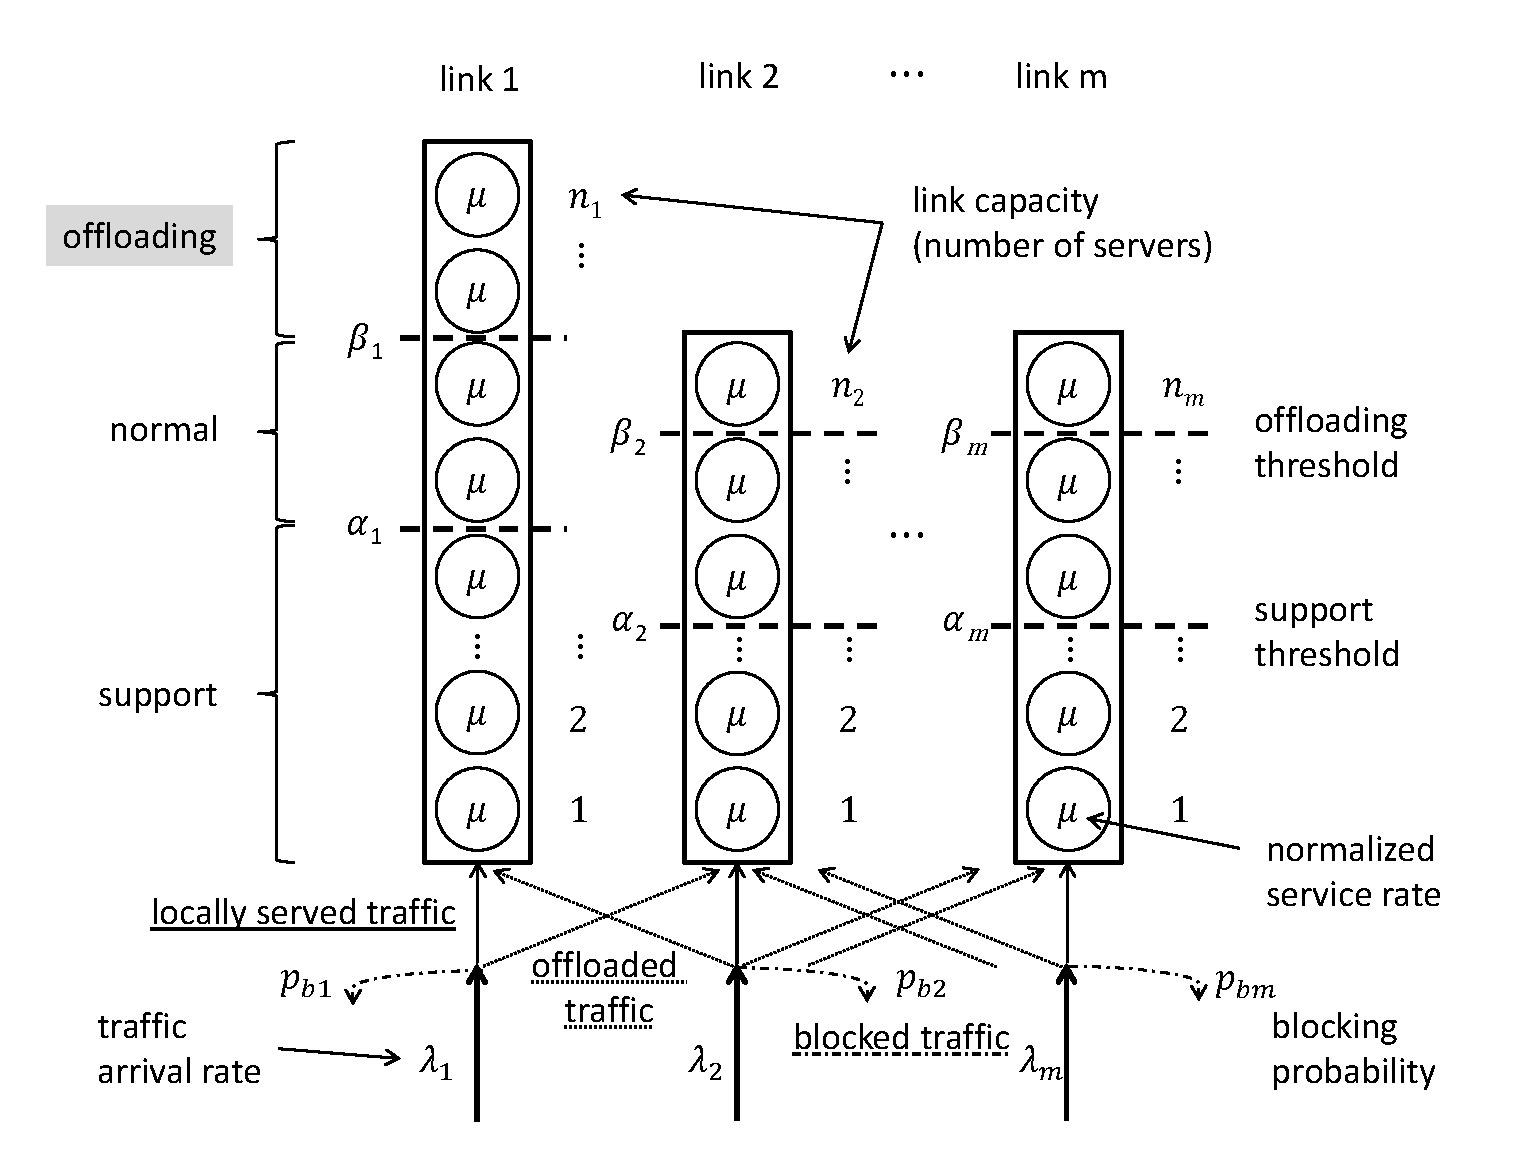
\includegraphics[width=0.9\textwidth]{aggregation/performance_model/figures/model_m}
  	\caption{System model.}
  	\label{fig:aggr:sysmodel}
\end{figure}

%In our scenario, we look at loaded access links on a short time scale. The throughput of each Internet connection is limited by a bottleneck (either on application side, on server side, or in the core Internet), such that the capacity of an access link cannot be fully utilized by a single connection. This means, each Internet connection will utilize a certain share of the access link bandwidth. The available capacity of a link $c$ is divided into a number $n$ of small atomic bandwidth fractions of equal size. This means, $c = n\cdot \xi$ with $\xi$ resembling the granularity of bandwidth allocation. For example, a $c=10\ \text{Mbps}$ link can be modeled as $n=20$ bandwidth fractions of $\xi=500\ \text{kbps}$ each, or also as $n=100$ bandwidth fractions of $\xi=100\ \text{kbps}$ each. For the remainder of this paper, we will consider $\xi$ as a global constant in the given scenario and model different capacities $c_i$ by assigning different $n_i$ to the links.
%short time frame load on links can be as stationary small variations poisson process

We consider the system in a short time frame, where the system load can be considered stationary.
Each access link is modeled as a multi-server blocking system, in which each server represents an available bandwidth fraction of the link.
Its utilization variations are modeled as a stationary process of singular and independent arrivals of traffic bursts, i.e., bandwidth fraction requests. This allows modeling an access link as M/M/n loss system \cite{kleinrock1975queuing}. We define $X$ as the random variable of the number of occupied bandwidth fractions on each backhaul link. It is modeled by a birth-death-process, in which bandwidth fractions are requested with Poisson arrivals at rate $\lambda$ and occupied for an negative-exponentially distributed service time with globally normalized rate $\mu=1$. Consequently, the load on each link is given by $\rho=\frac{\lambda}{n\cdot \mu}=\frac{\lambda}{n}$. The probability that $k$ bandwidth fractions are occupied in the considered M/M/n queue is $x(k)=P(X=k)$.

In the BeWifi approach (cf.~\refsec{sec:aggregation:background:aggr}), two thresholds are used, which define the bandwidth aggregation/offloading policy. The support threshold $\alpha$ indicates up to which percentage of utilization (i.e., number of own occupied bandwidth fractions) the system will offer bandwidth fractions to other systems. Furthermore, the offloading threshold $\beta$ with $\alpha\leq\beta$ sets the percentage of utilization above which the system will try to use bandwidth of other systems. According to these thresholds, a system can be in one of the following three macro states:

\begin{enumerate}
	\item \textit{support} ($0 \leq X < \lfloor\alpha\cdot n\rfloor$):\\ low utilization and offering bandwidth \, ,
	\item \textit{normal} ($\lfloor\alpha\cdot n\rfloor \leq X < \lfloor\beta\cdot n\rfloor$):\\ normal operation \, ,
	\item \textit{offloading} ($\lfloor\beta\cdot n\rfloor \leq X \leq n$):\\ high utilization and offloading to other systems \, .
\end{enumerate}

By applying the offloading policies, different Internet access links will collaborate and share traffic. More details on the investigated scenarios are presented in the following section.

Two bandwidth aggregation systems, i.e., systems offloading between $m$ access links, will be analyzed. First, we consider a bandwidth aggregation system with equal load on each access link. Moreover, a system in which one access link has a different load than the other $m-1$ links is modeled. As reference system we considered partitioned systems without offloading.% and a complete sharing system.

\subsection{Analysis of Reference Systems}

We compare the bandwidth aggregation gain of multiple collaborating Internet access links to a partitioned system without offloading. %, although it has to be noted that in many practical cases complete sharing is physically not possible.
The received bandwidth of each access link $E[X_i]$ and the blocking probability $p_{b_i}$ of each system $i$ are evaluated. The blocking probability gives the probability that the link is fully utilized and a bandwidth request of an application cannot be entirely satisfied. In practice, if TCP is used on the access link, the Internet connections throttle themselves and share the link equally. Depending on the used application and its characteristics, the application performance can then suffer, which can result in user dissatisfaction.

\subsubsection{Partitioned and Complete Sharing Systems}

For completely partitioned systems, i.e., $m$ different M/M/$n_i$ loss systems with arrival rates $\lambda_i,\ i\in\{1,\ldots, m\}$, the received bandwidths $E_0[X_i]$ can be computed individually for each access link by Little's Theorem as
\begin{equation}
E_0[X_i] = \frac{\lambda_i}{\mu}\cdot(1-p_{b_i}),% = \lambda_i\cdot(1-p_{b_i})\ ,
\end{equation}
in which we use the rate of accepted arrivals $\lambda_i\cdot(1-p_{b_i})$ and the globally normalized service rate $\mu=1$.

The blocking probability of partitioned systems $p_{b_i}$ follows from the Erlang-B formula \cite{kleinrock1975queuing}
\begin{equation}
p_{b_i} = \frac{\frac{(\frac{\lambda_i}{\mu})^{n_i}}{n_i!}}{\sum_{k=0}^{n_i}\frac{(\frac{\lambda_i}{\mu})^{k}}{k!}}\ .
\end{equation}

The performance $E_s[X]$ of a complete sharing system, i.e., a single M/M/n loss system with $n=\sum_{i=1}^m n_i$ servers and an arrival rate of $\lambda=\sum{i=1}^m \lambda_i$, can be computed by the same formulae.

\subsubsection{Approximations and Performance Metrics}

An approximation $\tilde{p}_b$ of the blocking probability $p_b$ can be calculated by the joint probability of a single system being fully occupied, while a separate single system is above the support threshold $\alpha$, i.e. could not help. If $X_1$ and $X_2$ are random variables for the number of jobs in system 1 and system 2, the joint probability is

\begin{equation}
\tilde{p}_b = P(X_1=n_1,X_2\geq \alpha\cdot n_2) = P(X_1=n_1)\cdot P(X_2\geq \alpha\cdot n_2)\ .
\end{equation}

Moreover, we analyze the mean total number of occupied bandwidth fractions $E[X]$% as well as the mean number of occupied bandwidth fractions $E[X_i]$ of each system
, which corresponds to the mean of total aggregated bandwidth. Following the same argumentation as above, $E[X]$ can be computed by Little's Theorem as
\begin{equation}
E[X] = \frac{\lambda_1+\lambda_2}{\mu}\cdot (1-p_b) = \frac{\lambda_1}{\mu}\cdot (1-p_{b_1})+\frac{\lambda_2}{\mu}\cdot(1-p_{b_2})\ .
\end{equation}

Finally, we take a look at the received bandwidth at each access link $E[X_{A_i}]$. Thereby, $X_{A_i}$ is a random variable for the number of bandwidth fractions (in all systems), which are occupied by arrivals from system $i$. It is obvious that $E[X_{A_i}] = E[X_i]
 = E_0[X_i]$ for the partitioned system. In case of offloading, $E[X_{A_i}]$ can be calculated from the mean total number of occupied bandwidth fractions by taking into account the share of accepted requests from each system.
\begin{equation}\label{equ:gain}
E[X_{A_i}] = \frac{\lambda_i(1-p_{b_i})}{\lambda_1(1-p_{b_1})+\lambda_2(1-p_{b_2})}\cdot E[X] = \frac{\lambda_i}{\mu}\cdot (1-p_{b_i})
\end{equation}

Nevertheless, it is the goal of bandwidth aggregation to cooperate in order to use spare capacity on access links to increase the received bandwidth where needed. Therefore, we can quantify the percentage of bandwidth gain for each system as
\begin{equation}
\omega_i = \frac{E[X_{A_i}]-E_0[X_i]}{E_0[X_i]}\ .
\end{equation}

\subsection{Simulation Description}
A discrete-event based simulation using arrival and departure events is implemented to validate the analytic model and to assess the system performance in more general cases. Each of the $m$ systems has a Poisson arrival process with rate according to its load. The service time of bandwidth fractions is exponentially distributed with mean 1. Offloading decisions are made according to the the number of occupied bandwidth fractions in the systems with respect to the support and offloading threshold. Therefore, the simulation state holds the requests being processed and the number of occupied bandwidth fractions for each system.
